\documentclass[a4paper,
12pt,
BCOR12mm,
]{scrartcl}
%scrreport
\usepackage[ngerman]{babel}
\usepackage[utf8]{inputenc}
\usepackage[T1]{fontenc}
\usepackage{url}
\usepackage[pdftex]{graphicx}
\usepackage{listingsutf8}
\usepackage{grffile}
\usepackage{epstopdf}
\usepackage{subfigure}
\usepackage[a4paper,left=23mm,right=23mm, top=33mm, bottom=66mm]{geometry}
% lstlisting settings
\lstset{
showspaces=false,
breaklines=true,
breakindent=0pt,
frame=single,
language=C,
extendedchars=true,
inputencoding=utf8/latin1,
identifierstyle=\ttfamily,
basicstyle=\tiny,
numbers=left,
numberstyle=\tiny,
}

\title{APUVS, Blatt 4}
\author{Jan Fajerski and Kai Warncke and Magnus Müller}

\begin{document}
% NOTE: compile with pdflatex --shell-escape main.tex

\maketitle 

\section*{Aufgabe 4.1}
\subsection{Testmaschine}
\begin{verbatim}
% uname -a
Linux centraldogma 2.6.35-ARCH #1 SMP PREEMPT Sat Oct 30 21:22:26 CEST 2010
	x86_64 Intel(R) Core(TM) i5 CPU M 520 @ 2.40GHz GenuineIntel GNU/Linux

% cat /proc/meminfo
MemTotal:        3848056 kB
MemFree:         1889880 kB
Buffers:          352748 kB
Cached:           541128 kB
[...]
\end{verbatim}

\begin{itemize}
	\item Quelltexte vgl. \pageref{src:sum} und \pageref{src:ascend}
	\item Stabilstes Ergebnis: 2-3 Threads.
	\item Mit 4 kann schneller sein, hat aber oft sehr starke Ausreißer --- daher nützt
		Mittelwertstimmung zur Abschätzung der Leistung auch relativ wenig (Varianz zu groß)
	\item Zeitanstieg annähernd linear. Anzahl der Threads bringt nur geringen Gewinn, mehr
		als 4 Threads werfen das Programm auf einen ähnlichen Zeitverbrauch wie bei der
		Verwendung nur eines Threads zurück.
	\item Muster in Graphik deutet auf starke Varianz hin, ähnelt aber dem Graph bei
		Verwendung der schnellsten Zeit (nicht beigefügt)
\end{itemize}

% some graphs
\begin{figure}[!h]
	\begin{center}
		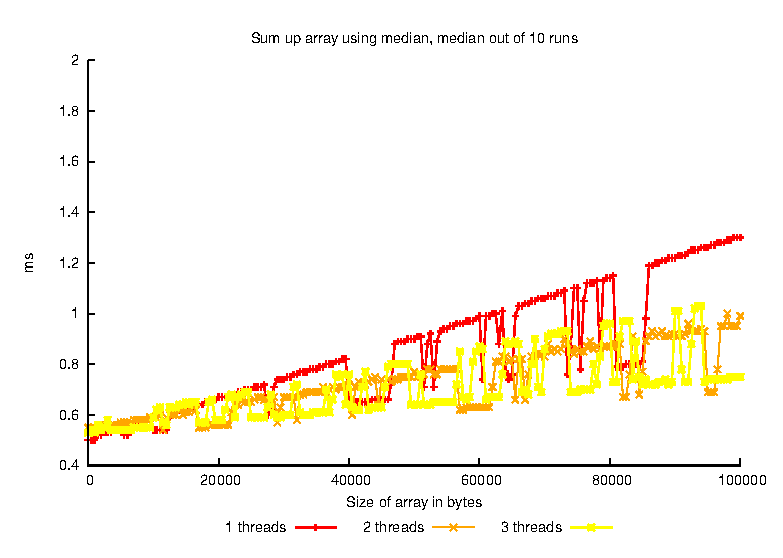
\includegraphics[width=0.5\textwidth]{../a_4_1/graphs/summation_median_1st}
	\end{center}
	\caption{Summation mit 1-3 Threads}
	\label{fig:summation_1_3}
\end{figure}
\begin{figure}[!h]
	\begin{center}
		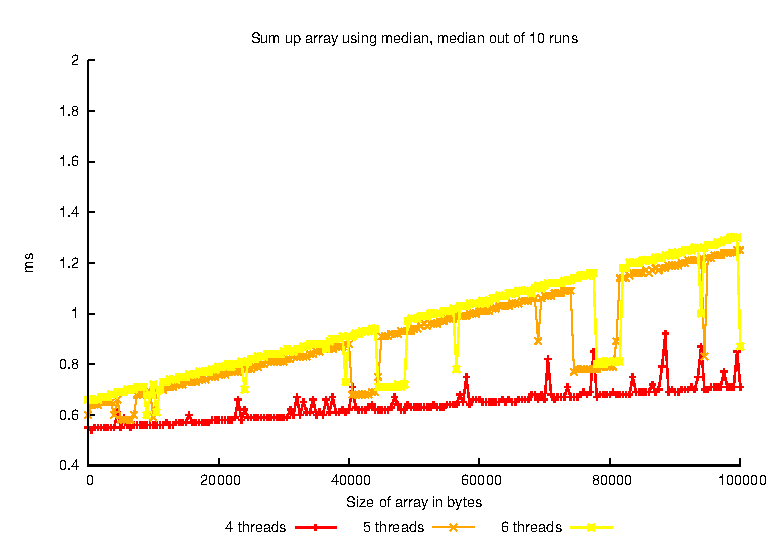
\includegraphics[width=0.5\textwidth]{../a_4_1/graphs/summation_median_2nd}
	\end{center}
	\caption{Summation mit 4-6 Threads}
	\label{fig:summation_4_6}
\end{figure}
\begin{figure}[!h]
	\begin{center}
		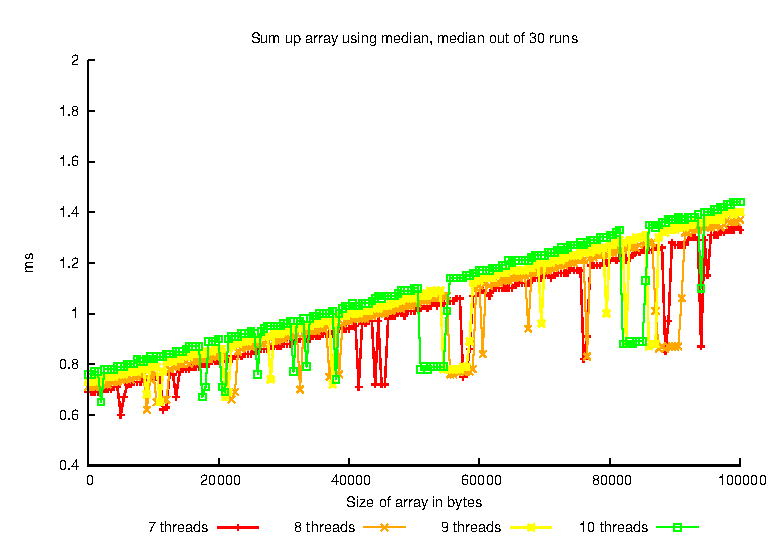
\includegraphics[width=0.5\textwidth]{../a_4_1/graphs/summation_median_3rd}
	\end{center}
	\caption{Summation mit 7-10 Threads}
	\label{fig:summation_7_10}
\end{figure}

\begin{figure}[!h]
	\begin{center}
		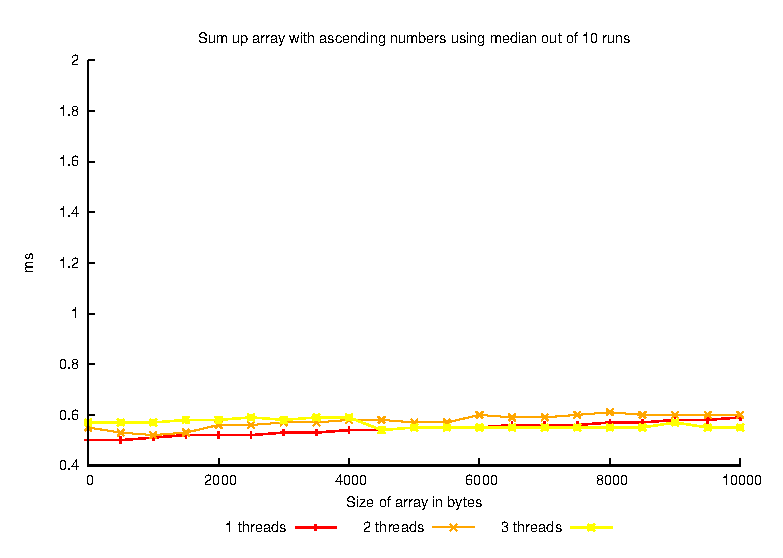
\includegraphics[width=0.5\textwidth]{../a_4_1/graphs/ascending_median_1st}
	\end{center}
	\caption{Summation aufsteigender Zahlen mit 1-3 Threads}
	\label{fig:ascending_1_3}
\end{figure}
\begin{figure}[!h]
	\begin{center}
		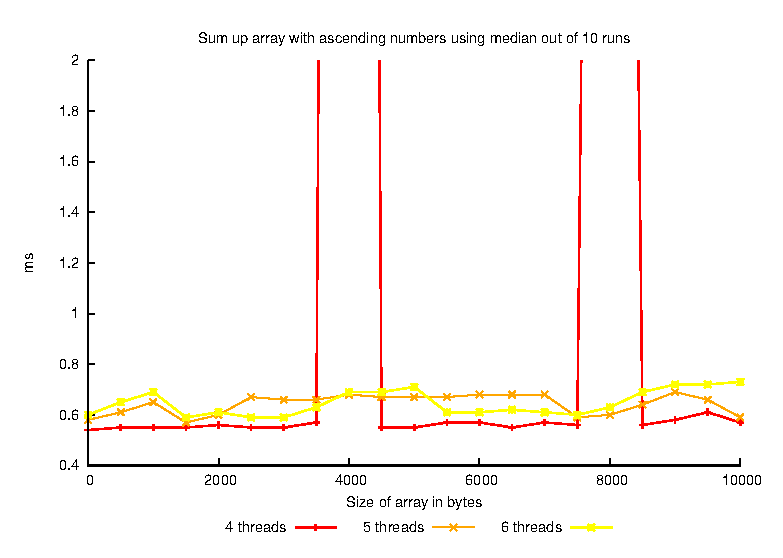
\includegraphics[width=0.5\textwidth]{../a_4_1/graphs/ascending_median_2nd}
	\end{center}
	\caption{Summation aufsteigender Zahlen mit 4-6 Threads}
	\label{fig:ascending_4_6}
\end{figure}
\begin{figure}[!h]
	\begin{center}
		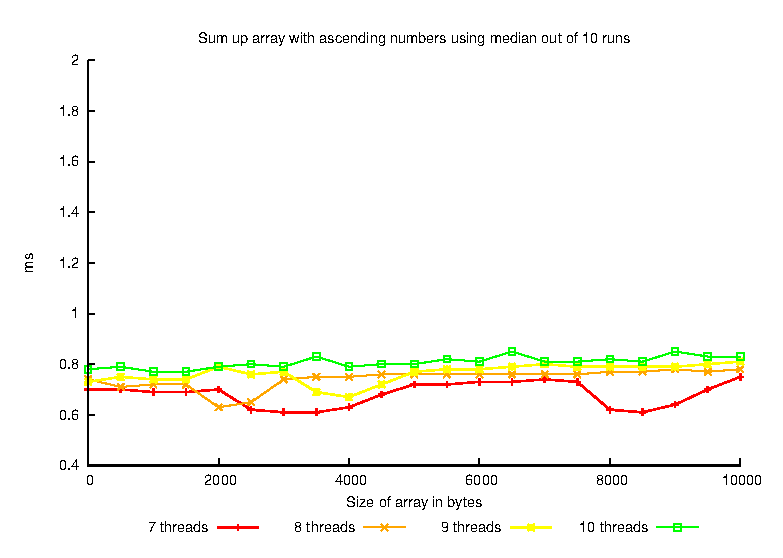
\includegraphics[width=0.5\textwidth]{../a_4_1/graphs/ascending_median_3rd}
	\end{center}
	\caption{Summation aufsteigender Zahlen mit 7-10 Threads}
	\label{fig:ascending_7_10}
\end{figure}


\pagebreak
\section*{Quelltexte}
\subsection*{Aufgabe 4.1}
\subsubsection{Einfache Summation}
\label{src:sum}
\lstinputlisting{../a_4_1/summation.c}
\subsubsection{Summation mit Array aufsteigender Zahlen}
\label{src:ascend}
\lstinputlisting{../a_4_1/summation_ascending_nums.c}

\subsubsection{Berechnung der Zeitdifferenz}
\label{src:messure}
\lstinputlisting{../a_4_1/messuretime.h}
\lstinputlisting{../a_4_1/messuretime.c}

\subsubsection{Ausgabefunktion}
\label{src:basic}
\lstinputlisting{../a_4_1/basic_functions.h}
\lstinputlisting{../a_4_1/basic_functions.c}

\end{document}
